\subsection{Representation and Evaluation}
\label{sec:genetic_programming:representation}
  As with GAs, the representation of the individuals is one of the most 
  important aspects of a GP.
  The representation is the encoding of potential solutions to the problem into
  a form that can be manipulated, executed and evaluated by the algorithm.

  Various methods exist for program representation, such as utilizing an abstract 
  syntax tree, a linear sequence of instructions, a stack of instructions, or a combination of these approaches.
  However, the most common representation is the \emph{tree representation}, where
  the program is represented as a composite data structure like the one shown in
  the introduction to this section.

  Let's consider the following problem: given a set of \(n\) points in the 
  plane, find the curve that best fits the points.
  This is a very common problem in statistics, and it is known as the
  \emph{symbolic regression} 
  problem~\autocite{kozaGeneticProgrammingProgramming1992a}.
  In this instance, we aim to conduct a symbolic regression of the function

  \begin{equation}
    f(x) = 5x^3 - 2x^2 + \sin(x) - 7;\; x \in [-1, 1]
  \end{equation}

  using this function, we can generate a set of random points in the curve as
  shown in \vref{fig:genetic_programming:representation:points} and 
  \vref{tab:genetic_programming:representation:points}.

  \begin{figure}[ht!]
    \centering
    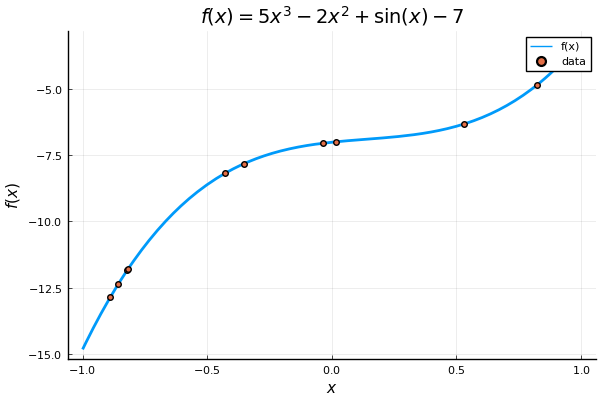
\includegraphics[width=0.6\textwidth]{img/theoretical_framework/symbolic.png}
    \caption{
      A set of points generated from the function \(5x^3 - 2x^2 + \sin(x) - 7\)
    }
    \label{fig:genetic_programming:representation:points}
  \end{figure}

  \begin{table}[ht!]
    \centering
    \begin{tabular}{|l|l|}
      \hline
      \(x\) & \(y\) \\
      \hline
      \hline
      -0.889160069272859    & -12.872628846869882 \\
      \hline
      -0.8561029711395651   & -12.358360817530986 \\
      \hline
      -0.8212951850355155   & -11.851004261287645 \\
      \hline
      -0.8181934125983823   & -11.807451940066528 \\
      \hline
      -0.4298586689110253   & -8.183442430668913  \\
      \hline
      -0.3523275114715019   & -7.812032934383372  \\
      \hline
      -0.0357759083395397   & -7.038557059091397  \\
      \hline
      0.017449673577553337  & -6.983133627817758  \\
      \hline
      0.5290096774879465    & -6.3148037734590945 \\
      \hline
      0.8211010511234629    & -4.848557205736884  \\
      \hline
    \end{tabular}
    \caption{
      A set of points generated from the function \(5x^3 - 2x^2 + \sin(x) - 7\)
    }
    \label{tab:genetic_programming:representation:points}
  \end{table}

  The next step would be to define the primitive set, that is the set of
  functions and terminals that will be used to build the programs.
  In this case, we will use the following set of functions and terminals:

  \begin{itemize}
    \item Functions:
      \begin{itemize}
        \item \(+\): Addition
        \item \(-\): Subtraction
        \item \(\times\): Multiplication
        \item \(/\): Division
        \item \(\sin\): Sine
        \item \(\cos\): Cosine
        \item \(\exp\): Exponential
        \item \(\log\): Logarithm
      \end{itemize}
    \item Terminals:
      \begin{itemize}
        \item \(x\): The variable \(x\)
        \item \(c\): An ephemeral constant
      \end{itemize}
  \end{itemize}

  Using this set of functions and terminals, we can represent the program as a
  tree, as shown in \vref{fig:genetic_programming:representation:tree}.

  \begin{figure}[ht!]
    \centering
    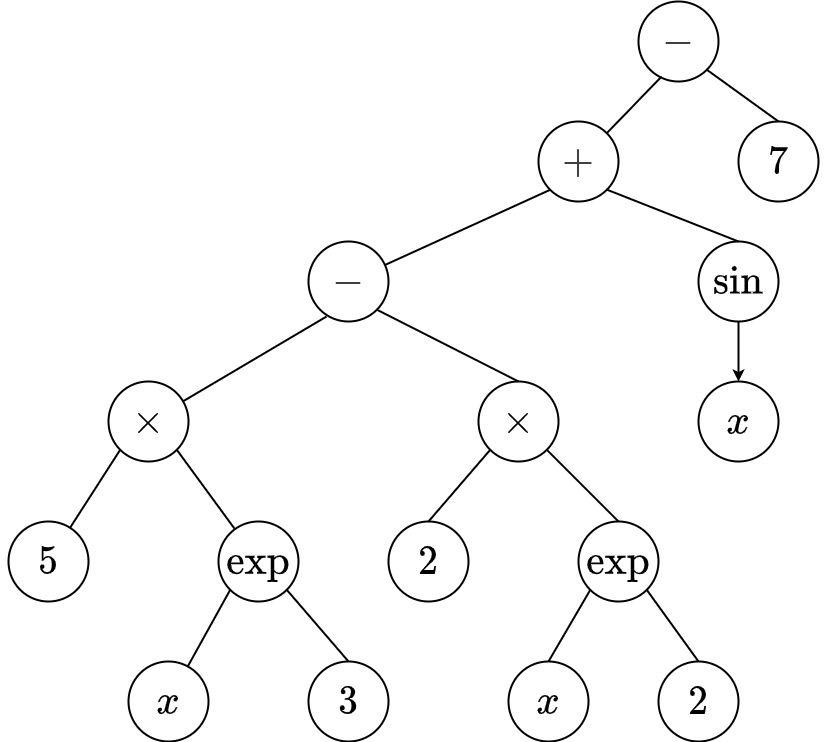
\includegraphics[width=0.5\textwidth]{img/theoretical_framework/Expected Expression Tree.png}
    \caption{
      A tree representation of the program \(5x^3 - 2x^2 + \sin(x) - 7\)
    }
    \label{fig:genetic_programming:representation:tree}
  \end{figure}

  Now, we need to define how to evaluate the fitness of a program.
  Again, there are many ways to do this, but a common way is to use the
  \emph{mean squared error} (MSE) between the points and the program.

  \begin{definition}[Mean Squared Error]
  \label{def:mse}
    If a vector of \(n\) predictions is generated from a sample of \(n\) data
    points on all variables, and \(\mathbf{y}_i\) is the \(i\)-th observed value
    and \(\hat{\mathbf{y}}_i\) is the \(i\)-th prediction, then the MSE of the 
    predictor is a function \(\mathrm{MSE}:\: \mathbb{R}^n \times \mathbb{R}^n
    \to \mathbb{R}\) defined as:

    \begin{equation}
      \label{eq:mse}
      \mathrm{MSE}(\mathbf{y}, \hat{\mathbf{y}}) 
        = \frac{1}{n} \sum_{i=1}^{n} (\mathbf{y}_i - \hat{\mathbf{y}}_i)^2
    \end{equation}
  \end{definition}

  The MSE is a common measure of the quality of an estimator, used in many
  \textit{machine learning} problems.

  In our case, we will use the MSE to evaluate the fitness of a program.
  Consider a program \(\mathsf{P}\) and two sets of points, \(\mathbf{x}\) and 
  \(\mathbf{y}\), as outlined in 
  \vref{tab:genetic_programming:representation:points}.
  Suppose also that \(\mathsf{P}[\mathbf{x}]\) is the set of points generated
  by evaluating \(\mathsf{P}\) on the points of \(\mathbf{x}\), and that
  \(\mathsf{P}(x)\) is the result of evaluating \(\mathsf{P}\) on the point
  \(x\).
  Then, we can define the fitness of \(\mathsf{P}\) as:

  \begin{equation}
  \label{eq:genetic_programming:representation:fitness}
    \phi_\mathsf{P} = \mathrm{MSE}(\mathbf{y}, \mathsf{P}[\mathbf{x}])
      = \frac{1}{n} \sum_{i=1}^{n} (\mathbf{y}_i - \mathsf{P}(\mathbf{x}_i))^2
  \end{equation}

  This section elucidated the pivotal aspects of Genetic Programming (GP), 
  focusing on representation of individuals and their evaluation.
  Individuals, potential solutions to a problem, can be encoded in several ways
  including tree representation.
  A common statistical problem, symbolic regression, was illustrated using a set
  of points on a curve from a function involving both polynomial and
  trigonometric elements.
  By defining a set of functions and terminals, these points were represented as
  a tree.
  The fitness of an individual program was assessed using the Mean Squared Error
  (MSE) between the points on the curve generated by the function and the points
  produced by the program.
  Thus, in the context of this problem, the fittest individual is the one that
  minimizes this error, i.e., best fits the curve.
  The methods described here underscore the versatility and applicability of GP
  to various types of problems.
  This method of representation and evaluation provides a robust basis for
  generating evolving populations of programs. 
  In the next sections we will discuss the mechanisms for generating these
  populations and the evolutionary operators that act on them.
